\chapter{Implémentation}

On programme la résolution de ce problème à l'aide de la bibliothèque Feel++. Pour commencer, on utilise une géomètrie d'un cylindre de rayon 0.05 et de longueur 0.5 orienté dans la direction $z$.
\begin{center}
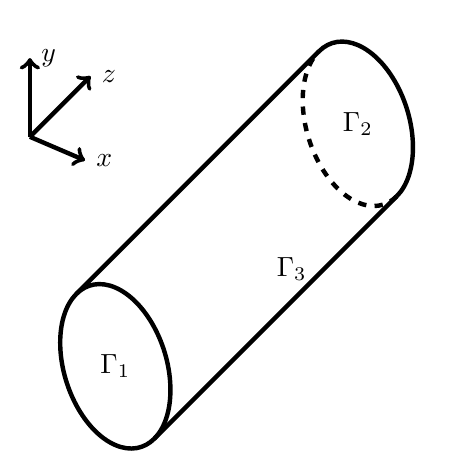
\begin{tikzpicture}
\begin{scope}[x={(.7cm,-.3cm)}]
\path (1,0,0);
\pgfgetlastxy{\cylxx}{\cylxy}
\path (0,1,0);
\pgfgetlastxy{\cylyx}{\cylyy}
\path (0,0,1);
\pgfgetlastxy{\cylzx}{\cylzy}
\pgfmathsetmacro{\cylt}{(\cylzy * \cylyx - \cylzx * \cylyy)/ (\cylzy * \cylxx - \cylzx * \cylxy)}
\pgfmathsetmacro{\ang}{atan(\cylt)}
\pgfmathsetmacro{\ct}{1/sqrt(1 + (\cylt)^2)}
\pgfmathsetmacro{\st}{\cylt * \ct}
\begin{scope}[every path/.style={ultra thick}]
\draw (0,0,0) circle[radius=1];
\draw[->] (-1,3,1) -- (0,3,1);
\draw (0,3,1) node [right] {$x$};
\draw[->] (-1,3,1) -- (-1,4,1);
\draw (-1,4,1) node [right] {$y$};
\draw[->] (-1,3,1) -- (-1,3,-1);
\draw (-1,3,-1) node [right] {$z$};
\draw (\ct,\st,0) -- ++(0,0,-8);
\draw (-\ct,-\st,0) -- ++(0,0,-8);
\draw (\ct,\st,-8) arc[start angle=\ang,delta angle=180,radius=1];
\draw[dashed] (\ct,\st,-8) arc[start angle=\ang,delta angle=-180,radius=1];
\draw (0,0,0) node {$\Gamma_1$};
\draw (0,0,-8) node {$\Gamma_2$};
\draw (1,0,-4) node {$\Gamma_3$};
\end{scope}
\end{scope}
\end{tikzpicture}
\end{center}

\section{Relèvement}

Dans le cas du cylindre, on a $\alpha_1=0$, ce qui conduit à ce que $\rot \mathbf{b}=0$ et donc $\mathbf{a}=\grad\psi^0$.

\subsection{Gradient dans $\HH^1$}
\label{impGradh1}

Si l'on veut utiliser le problème (\ref{pbpsi0}) dans $\HH^1$, alors il faut utiliser un multiplicateur de Lagrange pour ajouter une contrainte sur $\psi^0$, par exemple $\int \psi^0 = 0$. Cela se traduit par le changement de formulation variationnelle suivant où l'on cherche $(\psi^0,\lambda)\in \HH^1\times\R$ et où $(\varphi,\nu)$ est la fonction de test :
\[
\int_\Omega\grad \psi^0\grad\varphi + \int_\Omega \psi^0\nu + \int_\Omega \lambda\varphi = \int_{\partial\Omega} \alpha_0\varphi
\]
On va donc créé un espace de fonction produit correspondant à $\HH^1\times\R$.

\lstinputlisting[linerange={space}]{../../src/psi0.cpp}

On ajoute une fonction permettant de rajouter en option le profil d'entrée en fonction du rayon et de la vitesse. Cela correspond à $\alpha_0$.

\lstinputlisting[linerange={option}]{../../src/psi0.cpp}

Une fois les éléments de l'espace créé, on peut définir la forme bilinéaire de la façon suivante :

\lstinputlisting[linerange={bilinear}]{../../src/psi0.cpp}

Ici, $u$ correspond à $\psi^0$ et $v$ à $\varphi$.\\

On veut que ce qui rentre du cylindre par l'entrée, correspondant à la partie du maillage marquée 1, sorte par l'autre bout du cylindre, marqué 2, et que le tour du cylindre, marqué 3, soit imperméable. Ce qui donne la terme de droite suivant :

\lstinputlisting[linerange={rhs}]{../../src/psi0.cpp}

Une fois le problème résolut, on veut projeter le gradient de $\psi^0$ sur $\LL^2$. Pour cela on résout le problème simple $u=\grad\psi^0$.

\lstinputlisting[linerange={gradpsi0}]{../../src/psi0.cpp}

Le résultat est visible dans la section (\ref{respsih1}).

\subsection{Gradient dans $\HH(div)$}

\subsection{Rotationnel}

\section{Composante $z$}

Comme on se place dans le cylindre, on sait que $\bm{v}$ est colinéaires en tout point avec le vecteur de base $z$, ainsi on peut écrire $\bm{v}=(0,0,v^z)$.

\subsection{Sans relèvement}
\label{impZSR}

Dans cette section, on va supposer que l'on peut écrire $\bm{v}=\sum_i d_i \bm{h_i}$ où les $\bm{h_i}\in [H^1(\Omega)]^3$ sont solutions de :
\begin{align}
\rott\bm{h_i} &= \lambda^2_i \bm{h_i}\nonumber\\
\div \bm{h_i} &= 0 \label{eqhdiv}\\
\rot\bm{h_i}\cdot\bm{n}\big\rvert_{\Gamma_3} &= 0\nonumber
\end{align}
avec
\[
\bm{h_i}=
\begin{pmatrix}
0\\
0\\
h_i^z
\end{pmatrix}
\text{ et }
\rot\bm{h_i}=
\begin{pmatrix}
&\delta_y(h_i^z)\\
&-\delta_x(h_i^z)\\
&0
\end{pmatrix}
\]
Or, dans le cylindre, la vitesse ne dépend que de $x$ et de $y$, pas de $z$, et le vecteur normal est de la forme $\bm{n}=(n_x,n_y,0)$ sur $\Gamma_3$. Comme le cylindre est symétrique par rapport à l'axe $z$, on peut se ramener au cas où $\bm{n}=(1,0,0)$ ou $\bm{n}=(0,1,0)$, et donc on trouve que $h_i^z$ est une constante sur $\Gamma_3$. On peut prendre cette constante égale à 0.\\

De plus, la relation $\rott \mathbf{h} = \grad(\div \mathbf{h}) - \laplace \mathbf{h}$ et l'équation (\ref{eqhdiv}), permettent de remplacer le rotationnel du rotationnel par l'opérateur laplacien.\\
Comme on travail dans l'espace $[H^1(\Omega)]^3$ et non dans $[D^1(\Omega)]^3$, on a besoin de forcer la condition $\div\mathbf{g}=0$, pour cela, on utilise un terme de pression qui joue le rôle d'un multiplicateur de Lagrange. On a donc le problème suivant :
\begin{equation}
\left\{
\begin{aligned}
-\laplace\mathbf{h_i} + \grad p &= \Lambda \mathbf{h_i}\\
\div \mathbf{h_i}&=0\\
\rot\bm{h_i}\cdot\bm{n}\big\rvert_{\Gamma_3} &= 0
\end{aligned}
\right.
\end{equation}
En multipliant la première équation par $\bm{\varphi}\in [H^1(\Omega)]^3$ et la seconde par $q\in L^2(\Omega)$, on obtient la formulation faible suivante :
\begin{equation*}
\int_\Omega \overline{\grad\mathbf{h_i}}:\overline{\grad\bm{\varphi}} + p\div\bm{\varphi} + q\div\mathbf{h_i} = \lambda_i^2 \int_\Omega \mathbf{h_i}\cdot\bm{\varphi}
\end{equation*}
Et en utilisant le fait que $h_i=(0,0,h_i^z)$, le problème devient : trouver $(h_i^z,p)\in H^1(\Omega)\times H^1(\Omega)$ tel que, $\forall (\varphi,q)\in H^1(\Omega)\times H^1(\Omega)$ :
\[
\int_\Omega \partial_x h_i^z \partial_x\varphi + \partial_y h_i^z \partial_y\varphi + \partial_z h_i^z \partial_z\varphi + \varphi\grad p + h_i^z\grad q = \lambda_i^2 \int_\Omega h_i^z\varphi
\]
avec $h_i^z = 0$ sur $\Gamma_3$.\\

On utilise donc des éléments de Lagrange d'ordre 2 pour $h_i^z$ et des éléments de Lagrange d'ordre 1 pour $p$.
\lstinputlisting[linerange={typedef}]{../../src/eigenlapZ.h}

On obtient le terme de gauche avec ces lignes de codes :
\lstinputlisting[linerange={formA,nrelev}]{../../src/eigenlapZ.cpp}

Et le terme de droite :
\lstinputlisting[linerange={formB}]{../../src/eigenlapZ.cpp}

\subsubsection{Décomposition}

Afin de décomposer $\bm{h_i}$, on utilise la même formulation que pour $\bm{g_i^0}$ et $\psi_i$. Ce qui donne :
\lstinputlisting[linerange={gi0}]{../../src/eigenlapZ.cpp}
\lstinputlisting[linerange={psi}]{../../src/eigenlapZ.cpp}
Cette partie est assez délicate, car les conditions aux bords ne devrait pas être les mêmes pour $\bm{h_i}$ et $\bm{g_i}$.\\

Les résultats de cette implémentation sont présenté dans \ref{resZSR}.

\subsection{Avec relèvement}
\label{impZAR}

Ici, on utilise le relèvement, $\bm{v}=\bm{a}+\bm{u}$ avec $\bm{u}=\sum_i c_i\bm{g_i}$ où les $\bm{g_i}\in [D^1(\Omega)]^3$ sont solutions de :
\begin{align*}
\rott  \mathbf{g_i} &= \Lambda_i \mathbf{g_i}\\
\mathbf{g_i}\cdot \mathbf{n}\restr &= 0\\
\rot \mathbf{g_i}\cdot \mathbf{n}\restr &= 0\\
\rott  \mathbf{g_i}\cdot \mathbf{n}\restr &= 0
\end{align*}
avec
\[
\bm{g_i}=
\begin{pmatrix}
0\\
0\\
g_i^z
\end{pmatrix}
\text{ et }
\rot\bm{g_i}=
\begin{pmatrix}
&\delta_y(g_i^z)\\
&-\delta_x(g_i^z)\\
&0
\end{pmatrix}
\]
De la même manière que dans \ref{impZSR}, on utilise le laplacien à la place du rotationnel et un terme en pression pour forcer la pression nulle.\\

Sur $\Gamma_1$ et $\Gamma_2$, $\bm{n}=(0,0,\pm 1)$, et donc la condition $\bm{g}\cdot \bm{n}=0$ conduit à $g_3 = 0$.\\
Donc $\bm{g}=0$ sur $\partial\Omega$.\\

Ainsi le terme de droite dans la formulation se traduit par :
\lstinputlisting[linerange={formA,relev}]{../../src/eigenlapZ.cpp}

\subsection{Problème spectral}
\label{impZPS}

Comme les fonctions de bases sont de la forme $\bm{g_i}=(0,0,g_i^z)$, on a que $\bm{g_i}\times\bm{g_i}=0$, ainsi, le terme non linéaire est nul.\\

De même, 
\[
\bm{a}\times\bm{g_i}=\begin{pmatrix}
a_xg_i^z\\
-a_yg_i^z\\
0
\end{pmatrix}
\text{ et donc }
(\bm{a}\times\bm{g_i})\cdot\bm{g_k} = \begin{pmatrix}
a_xg_i^z\\
-a_yg_i^z\\
0
\end{pmatrix}\cdot\begin{pmatrix}
0\\
0\\
g_k^z
\end{pmatrix} = 0
\]
Ainsi, pour trouver les coefficients $d_k$ ou $c_k$, il n'y a qu'à calculer les coefficients suivants :
\[
c_k = \frac{Re\times (\bm{f},\bm{g_k})+\langle \alpha_2,\psi_k\rangle}{\lambda_k^2}
\]

Pour cela on calcule d'abord tous les coefficients $(\bm{f},\bm{h_k})\ \forall k=0,\dots,M$
\lstinputlisting[linerange={rfk}]{../../src/spectralproblem.cpp}

Puis les coefficients $\langle\alpha_2,\psi_k\rangle\ \forall k=0,\dots,M$
\lstinputlisting[linerange={rpk}]{../../src/spectralproblem.cpp}

Ainsi, il ne reste plus qu'à calculer les $d_k\ \forall k=0,\dots,M$
\lstinputlisting[linerange={spz}]{../../src/spectralproblem.cpp}

\section{Cas général}

\subsection{Modes propres}

Ici on veut utiliser les travaux de V. Girault \cite{Girault90-1}, pour justifier l'utilisation des éléments de Nedelec. Pour cela, on a besoin de définir l'espace \[X = \{\bm{v}\in H(rot)\ |\ (\rot\bm{v}\cdot\bm{n})\restr=0 \}\]
On rappel les définitions suivantes :
\begin{align*}
L^2_\sigma(\Omega) &= \{\mathbf{v} \in L^2(\Omega)\ |\ \div \mathbf{v} = 0\text{ et }\mathbf{v}\cdot \mathbf{n}\restr = 0 \}\\
D^1(\Omega) &= \{\mathbf{v} \in H^1(\Omega)\cap L^2_\sigma(\Omega)\ |\ (\rot \mathbf{v}\cdot \mathbf{n})\restr = 0  \}
\end{align*}
De plus, on a (voir \cite{Girault79}) :
\[
H^1(\Omega)=H(rot)\cap H(div)
\]
D'où:
\begin{align*}
D^1(\Omega) &= \{\bm{v}\in H^1(\Omega)\cap L^2_\sigma(\Omega)\ |\ (\rot \mathbf{v}\cdot \mathbf{n})\restr = 0  \}&\\
&=\{\bm{v}\in H(rot)\cap H(div)\cap L^2_\sigma(\Omega)\ |\ (\rot \mathbf{v}\cdot \mathbf{n})\restr = 0  \}&\\
&&\text{ or }L^2_\sigma\subset H(div)\\
&=\{\bm{v}\in H(rot)\cap L^2_\sigma(\Omega)\ |\ (\rot \mathbf{v}\cdot \mathbf{n})\restr = 0  \}&\\
&=\{\bm{v}\in H(rot)\ |\ (\rot \mathbf{v}\cdot \mathbf{n})\restr = 0  \}\cap L^2_\sigma(\Omega)&\\
&=X\cap L^2_\sigma(\Omega)&
\end{align*}


Le problème aux valeurs propres est :\\
Trouver $(\bm{g},\lambda)\in X\cap L^2_\sigma\times\R$ tel que :
\begin{align}
\rott\bm{g}&=\lambda^2\bm{g} \label{impPb1}\\
\div\bm{g}&=0 \label{impPb2}\\
(\bm{g}\cdot\bm{n})\restr&=0 \label{impPb3}\\
(\rot\bm{g}\cdot\bm{n})\restr&=0 \label{impPb4}\\
(\rott\bm{g}\cdot\bm{n})\restr&=0 \label{impPb5}
\end{align}
Mais les conditions (\ref{impPb2}-\ref{impPb3}) sont satisfaites par le fait que $\bm{g}\in L^2_\sigma$ et la condition (\ref{impPb4}) par l'appartenance à $X$.\\

En passant à la forme variationnelle, on impose la condition (\ref{impPb5}), voir le chapitre (\ref{eigen}). On a donc le problème suivant :\\
Trouver $(\bm{g},\lambda)\in X\cap L^2_\sigma\times\R$ tel que $\forall \bm{\varphi}\in X\cap L^2_\sigma$ :
\[
\int_\Omega (\rot\bm{g})\cdot(\rot\bm{\varphi}) = \lambda^2\int_\Omega \bm{g}\cdot\bm{\varphi}
\]

Ne pouvant pas utiliser directement des fonctions de bases à divergence nulle pour les éléments finis, on impose cette condition par un terme de pression fictif. On a donc :\\
Trouver $((\bm{g},p),\lambda)\in X\cap L^2_\sigma \times H^1 \times \R$ tel que $\forall (\bm{\varphi},q)\in X\cap L^2_\sigma \times H^1$ :
\begin{align*}
\int_\Omega (\rot\bm{g})\cdot(\rot\bm{\varphi}) + \int_\Omega\bm{\varphi}\grad p &= \lambda^2\int_\Omega \bm{g}\cdot\bm{\varphi}\\
\int_\Omega (\div\bm{g}) q &= 0
\end{align*}
En intégrant par partie la seconde équation, on obtient
\[
\int_\Omega (\div\bm{g}) q = \int_\Omega \bm{g}\grad q - \int_{\partial\Omega} (\underbrace{\bm{g}\cdot \bm{n}}_{=0})q = 0
\]
On peut donc imposer les contraintes (\ref{impPb2}-\ref{impPb3}), liées à $L^2_\sigma$, dans la formulation faible suivante :\\
Trouver $((\bm{g},p),\lambda)\in X \times H^1 \times \R$ tel que $\forall (\bm{\varphi},q)\in X \times H^1$ :
\[
\int_\Omega (\rot\bm{g})\cdot(\rot\bm{\varphi}) + \int_\Omega\bm{\varphi}\grad p + \int_\Omega \bm{g}\grad q = \lambda^2\int_\Omega \bm{g}\cdot\bm{\varphi}
\]

Pour imposer la condition (\ref{impPb4}), on utilise une méthode de pénalisation, le problème devient donc :
Trouver $((\bm{g},p),\lambda)\in H(rot) \times H^1 \times \R$ tel que $\forall (\bm{\varphi},q)\in H(rot) \times H^1$ :
\[
\int_\Omega (\rot\bm{g})\cdot(\rot\bm{\varphi}) + \int_\Omega\bm{\varphi}\grad p + \int_\Omega \bm{g}\grad q + \gamma\int_{\partial\Omega}(\rot\bm{g_i}\cdot\bm{n})(\rot\bm{\varphi}\cdot\bm{n}) = \lambda^2\int_\Omega \bm{g}\cdot\bm{\varphi}
\]
avec $\gamma$ une très grande valeur.


\iffalse

On va utiliser une classe \texttt{EigenProblem} acceptant des problèmes de plusieurs dimensions, dans notre cas le problème est de dimension 3.\\
Pour commencer, on va définir l'espace de fonctions, pour cela on va dire au programme que l'on utilise des simplexes, et que la maillage devra être fait de cette manière.\\
Puis comme on veut utiliser chaque composante de la solution pour décrire la normale égale à 0, on va créer une base de fonctions où l'on pourra accéder à chaque composante, chacune sera des fonctions de Lagrange d'ordre 2 scalaire.\\
On utilise enfin la base et le type de maillage pour créer l'espace de fonctions.

\lstinputlisting[linerange={typedef}]{../../src/mode_gen_curl.cpp}

On lit ensuite le nombre de valeurs propres que l'on veut et le nombre de valeurs propres convergées, qui doit être supérieur au premier, dans le fichier de configuration qui doit être nommé de la même manière que l'application. Dans ce fichier doit se trouver aussi le nom du fichier contenant la géographie utilisée, ou le maillage récupérer depuis HyperMesh. On importe cette géographie ou ce maillage avec la fonction \texttt{loadMesh}.

\lstinputlisting[linerange={option,mesh}]{../../src/mode_gen_curl.cpp}

Puis, on a plus qu'à créer un espace de fonction du type précédemment défini, et récupérer deux éléments de cet espace, puis prendre les 3 composantes de ces éléments.

\lstinputlisting[linerange={space}]{../../src/mode_gen_curl.cpp}

Il faut ensuite construire une forme bilinéaire $a$ correspondant à $\int_\Omega curl\ g\cdot curl\ \psi\ dX$. On utilise donc pour cela le fait que $curl\ u = (\partial_y(u_3)-\partial_z(u_2))\vec{i} + (\partial_z(u_1) - \partial_x(u_3))\vec{j} + (\partial_x(u_2)-\partial_y(u_1))\vec{k}$.\\
De plus, on utilise un terme de stabilisation de type $div \times div$. Ce terme ne doit pas jouer de rôle significatif, car la divergence doit tendre vers 0. Il permet seulement d'inverser la matrice A.

\lstinputlisting[linerange={bilinear}]{../../src/mode_gen_curl.cpp}

Puis, on traduit $g\cdot n\big\rvert_{\partial\Omega}=0$ par le fait que $z=0$ sur les deux extrémités du cylindre et que $x=y=0$ sur le tour du cylindre.

\lstinputlisting[linerange={boundary}]{../../src/mode_gen_curl.cpp}

On crée ensuite le second terme correspondant à $\int_\Omega g\cdot\psi\ dX$.

\lstinputlisting[linerange={rhs}]{../../src/mode_gen_curl.cpp}

On peut maintenant résoudre le problème aux valeurs propres. On utilise pour cela la librairie \href{http://www.grycap.upv.es/slepc/}{SLEPc}, qui va utiliser un algorithme de type Krylov-Schur(\ref{arnoldi}) pour trouver \texttt{nev} valeurs propres, en se servant de \texttt{ncv} vecteurs pour la base du sous-espace de Krylov. On crée donc 2 matrices avec les formes bilinéaires précédemment construites, et on indique que l'on cherche les valeurs propres de plus petite magnitute.

\lstinputlisting[linerange={modes}]{../../src/mode_gen_curl.cpp}

Enfin, pour visualiser les résultats, on utilise un élément d'un espace vectoriel qui est le projeté du vecteur formé par les composantes de la solution.

\lstinputlisting[linerange={project}]{../../src/mode_gen_curl.cpp}

Les résultats sont visibles dans le chapitre \ref{resModes}.

\fi

\subsection{Problème spectral}

On peut maintenant résoudre le problème (\ref{fvspec}).\\
Cette équation comporte le terme
\[
\sum_i\sum_j c_i\lambda_i c_j(\mathbf{g_i}\times \mathbf{g_j}, \mathbf{g_k})
\]
qui est non linéaire. Ce problème s'écrit donc sous la forme :
\[
F(c) = 0
\]
où $F:\R^M\rightarrow\R^M$, $c=(c_1,\ldots, c_M)$ et :
\begin{align*}
F_k(c) &= \frac{1}{Re} c_k\lambda_k^2 + \sum_i c_i\lambda_i(\mathbf{g_i}\times \mathbf{a}, \mathbf{g_k})\\
&+ \sum_{i,j} c_i\lambda_i c_j (\mathbf{g_i}\times \mathbf{g_j}, \mathbf{g_k}) - (\mathbf{h_a},\mathbf{g_k}) - \frac{1}{Re}\langle \alpha_2, \psi_k \rangle
\end{align*}

On va utiliser une méthode de Newton pour résoudre ce problème, on cherche donc :
\begin{equation}
\label{Newton}
c^{(l+1)} = c^{(l)} - J(c^{(l)})^{-1}F(c^{(l)})\quad l=0,1,\ldots
\end{equation}
où $c^{(0)}$ est une donnée initiale et $J(c)$ est la matrice jacobienne de $F$ en $c$ :
\[
J(c)=
\begin{pmatrix}
\frac{\partial F_1(c)}{\partial c_1} & \ldots & \frac{\partial F_1(c)}{\partial c_M}\\
\vdots & \ddots & \vdots\\
\frac{\partial F_M(c)}{\partial c_1} & \ldots & \frac{\partial F_M(c)}{\partial c_M}
\end{pmatrix}
\]
avec 
\begin{align*}
J(c)_{ki} = \frac{\partial F_k(c)}{\partial c_i} &= \delta_{ki}\lambda_i^2 + \lambda_i(\mathbf{g_i}\times \mathbf{a},\mathbf{g_k})\\
&+ \sum_j\lambda_i c_j (\mathbf{g_i}\times\mathbf{g_j},\mathbf{g_k}) + \sum_j c_j\lambda_j (\mathbf{g_j}\times\mathbf{g_i},\mathbf{g_k})
\end{align*}
Résoudre (\ref{Newton}) est équivalent à résoudre 
\begin{equation}
\label{INewton}
\begin{aligned}
J(c^{(l)})\delta c^{(l)} = -F(c^{(l)})\\
c^{(l+1)}=c{(l)}+\delta c^{(l)}
\end{aligned}
\end{equation}

Toutefois, résoudre exactement (\ref{INewton}) à chaque itération peut être très couteux et peu intéressant, surtout au début lorsque l'on est loin de la solution exacte. On utilise donc une méthode de Newton inexacte pour résoudre cette équation à chaque itération.\\
Cette méthode est elle même une méthode itérative, et la précision de la méthode dépend du nombre d'itération, ainsi, plus on se rapproche de la solution exacte, plus on veut être précis.
\\On se donne donc une suite de nombres positifs $(\eta_l)$, et les itérations continuent jusqu'à ce que :
\[
\frac{||r_l^{(i)}||}{||F(c^{(l)})||} \leq \eta_l<1
\]
où
\[
r_l^{(i)} = J(c^{(l)})\delta c^{(l,i)} + F(c^{(l)})
\]

\iffalse

\subsection{Composantes $(x,y,z)$}
Si l'on ne suppose pas $\bm{g}=(0,0,g_3)$, on a : 
\[
\bm{g}=
\begin{pmatrix}
g_1\\
g_2\\
g_3
\end{pmatrix}
\text{ et }
\rot\bm{g}=
\begin{pmatrix}
\delta_y(g_3)-\delta_z(g_2)\\
\delta_z(g_1)-\delta_x(g_3)\\
\delta_x(g_2)-\delta_y(g_1)
\end{pmatrix}
\]

La condition $\bm{g}\cdot\bm{n}=0$ mène sur l'entrée et la sortie, de la même manière que dans \ref{freefem1d} à $g_3=0$, tandis que sur le tour du cylindre, on peut prendre $g_1=g_2=0$ pour satisfaire cette condition.\\

On peut utiliser la contrainte $\div\bm{g}=0$, qui est continue sur les bords, donc applicables sur le tour du cylindre, pour contraindre $g_3$. Comme sur le tour, $g_1=g_2=0$, on a que $\div\bm{g}=\delta_z(g_3)=0$, donc $g_3$ est une constante sur le tour du cylindre, on peut prendre cette constante égale à 0.\\

La condition $\rot\bm{g}\cdot\bm{n}=0$, sur l'entrée et la sortie se lit $\delta_x(g_2)=\delta_y(g_1)$, toujours de la même façon, prendre $g_1$ constant et $g_2$ constant permet de satisfaire la condition.\\

Comme toutes ces contraintes s'expriment par le fait que $\bm{g}$ doit être une constante, on peut choisir cette constante, par exemple, $\bm{g}=0$.

\fi


%%% Local Variables:
%%% TeX-master: "../report.tex"
%%% End:
